\section{The Error-Delay Curve}
\label{delayErrorCurve}

In Section \ref{controlProblem}, we postulated the existence of an Estimation Error vs Computation Delay curve (the `error-delay curve').
This curve is used at every time step by the controller to determine the operating point $(\delta, \epsilon)$ for the next time step.
In this section we demonstrate how such a curve may be obtained for particular applications. 
Specifically, we consider a visual perception tool chain, where each tool of the tool chain has a knob that tunes its performance.
These knobs can be used to profile the tool chain and obtain its error-delay curve on particular platforms.
Because power consumption is correlated to computation time, the error-delay curve can also be viewed as an error-power curve.
The power consumption of the estimator task can be modeled using the $\alpha$ term of Eq.??.
Thus, the controller can save power by selecting operating modes $(\delta,\epsilon)$ that achieve the control objectives at a lower energy cost.

The first perception algorithm we consider is the FAST corner detector~\cite{rosten_2006_machine}.
Corners in an image can be tracked across video frames to perform self-localization by a moving robot. 
Thus it is important to detect corners at frame rate or faster, to provide a timely state estimate to the control algorithm.
The number $\#C$ of corners detected in a frame directly affects the runtime of the corner detector and the quality of the state estimate.
Generally speaking, detecting more corners requires a longer runtime, and results in better self-localization, \emph{assuming acceptable quality of the detected corners}.
If the additional corners are of poor quality (i.e., hard to track across frames), then we can expect the self-localization error to actually increase.
Thus the number $\#C$ of corners is a knob which can be varied to obtain an error-delay curve for self-localization with corner detection. 

Fig.~\ref{fig:fast} shows the error-delay curve of self-localization error using the FAST corner detector~\cite{rosten_2006_machine}.
The curve was obtained on an Odroid U3 [??], which is a quadcore \hatodoin{complete odroid specs}.
For each value of the knob $\#C$ (i.e., each requested number of corners), we ran the corner detector on a video sequence shot by a downward facing camera on-board a hexarotor while flying certain pre-set patterns.
The corners and some auxiliary data are then fed to a self-localization algorithm.
Ground truth for computing the self-localization error was obtained from the Vicon system which \hatodoin{half-sentence on what vicon does.}
As we repeat each flight several times, this results in a distribution of $(\delta,\epsilon)$ values for each value of $\#C$. 
We retained the $90^{th}$ percentile values for $\delta$ and $\epsilon$, since these are used as worst-case estimates by the controller of Section \ref{controlProblem}.
It can be seen that a larger number of requested corners produces a smaller estimation error and longer runtime.
Starting at 250 corners, the error increases, however.
We hypothesize this is due to the decreasing quality of the corners being returned by FAST.
\begin{figure}[t]
\centering
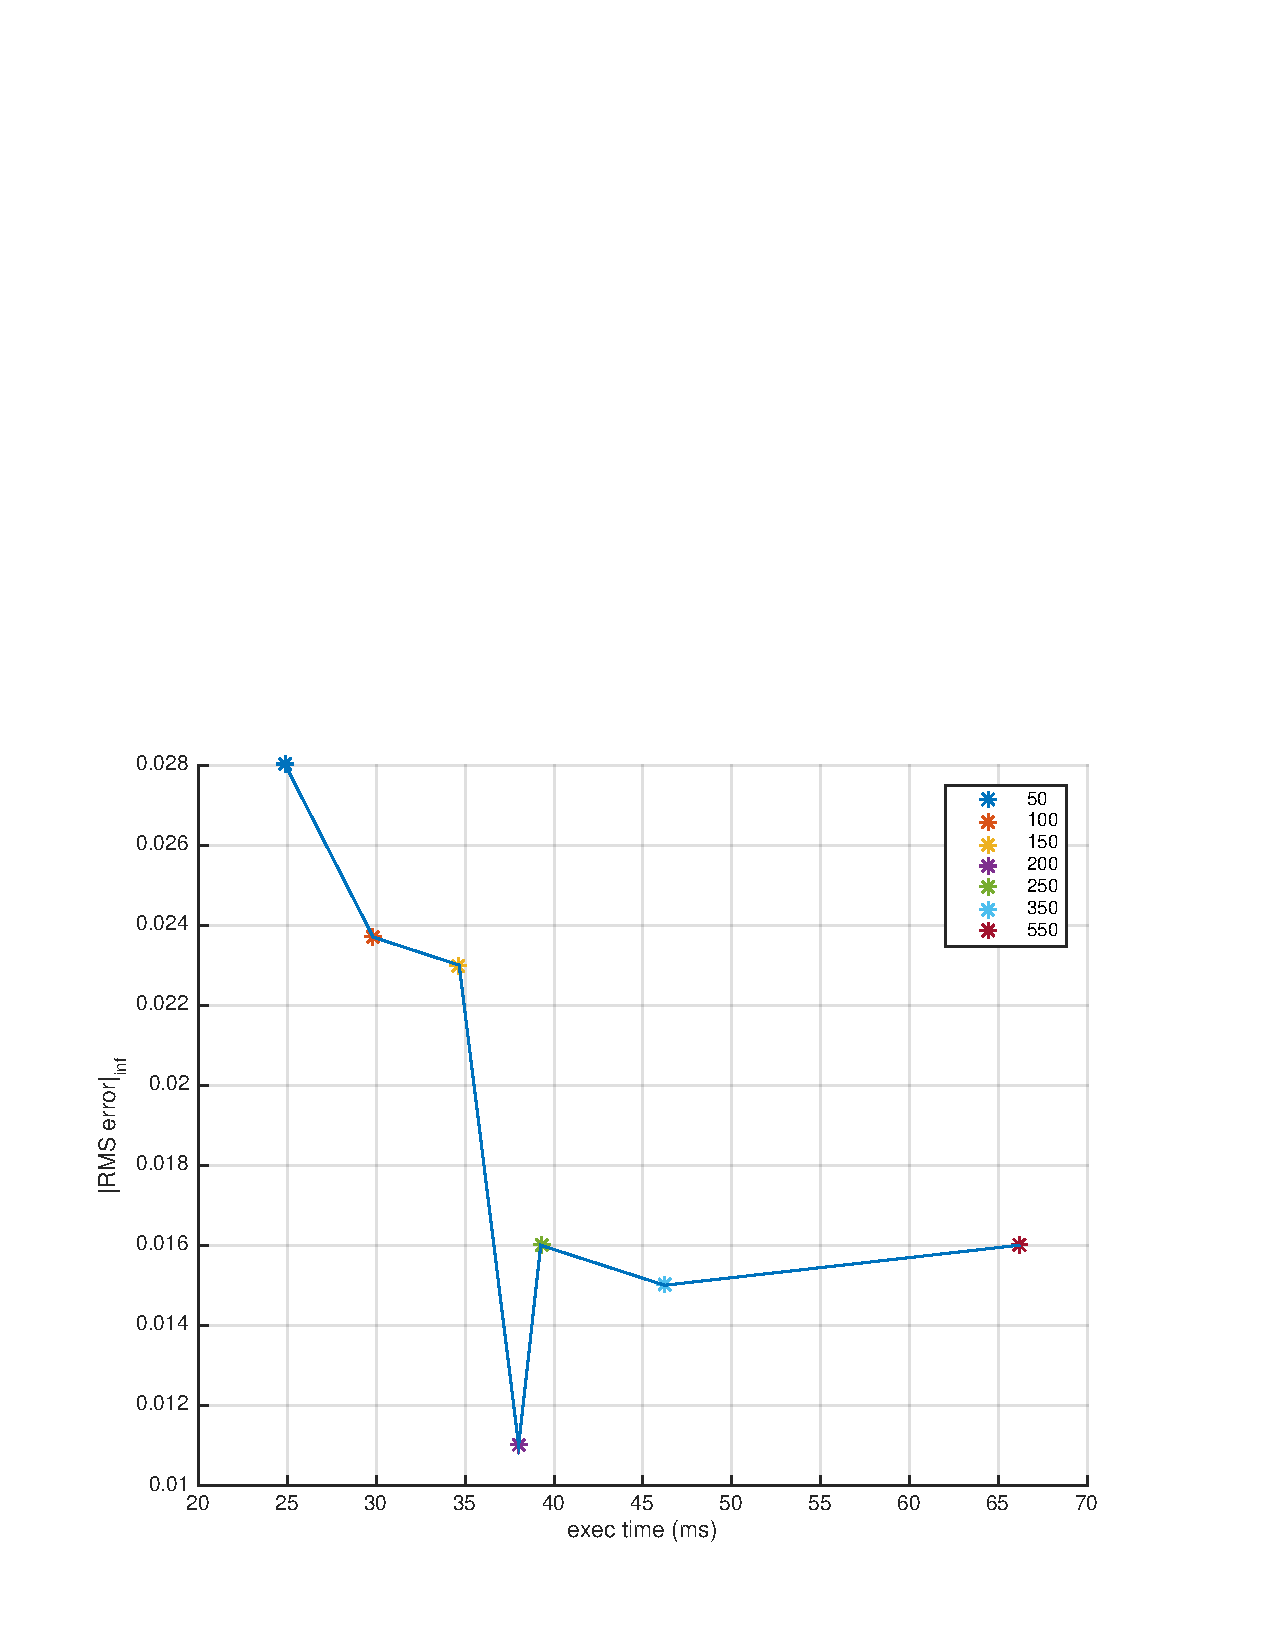
\includegraphics[width=0.7\linewidth]{figures/init_eps_delta_90th}
\caption{Error-delay curve for the FAST corner detector running on the Odroid U3}
\label{fig:fast}
\end{figure}

Fig.~\ref{fig:fastErrVsPower} shows the power consumption vs estimation error, which correlates well with Fig.~\ref{fig:fast}.
\begin{figure}[t]
	\centering
	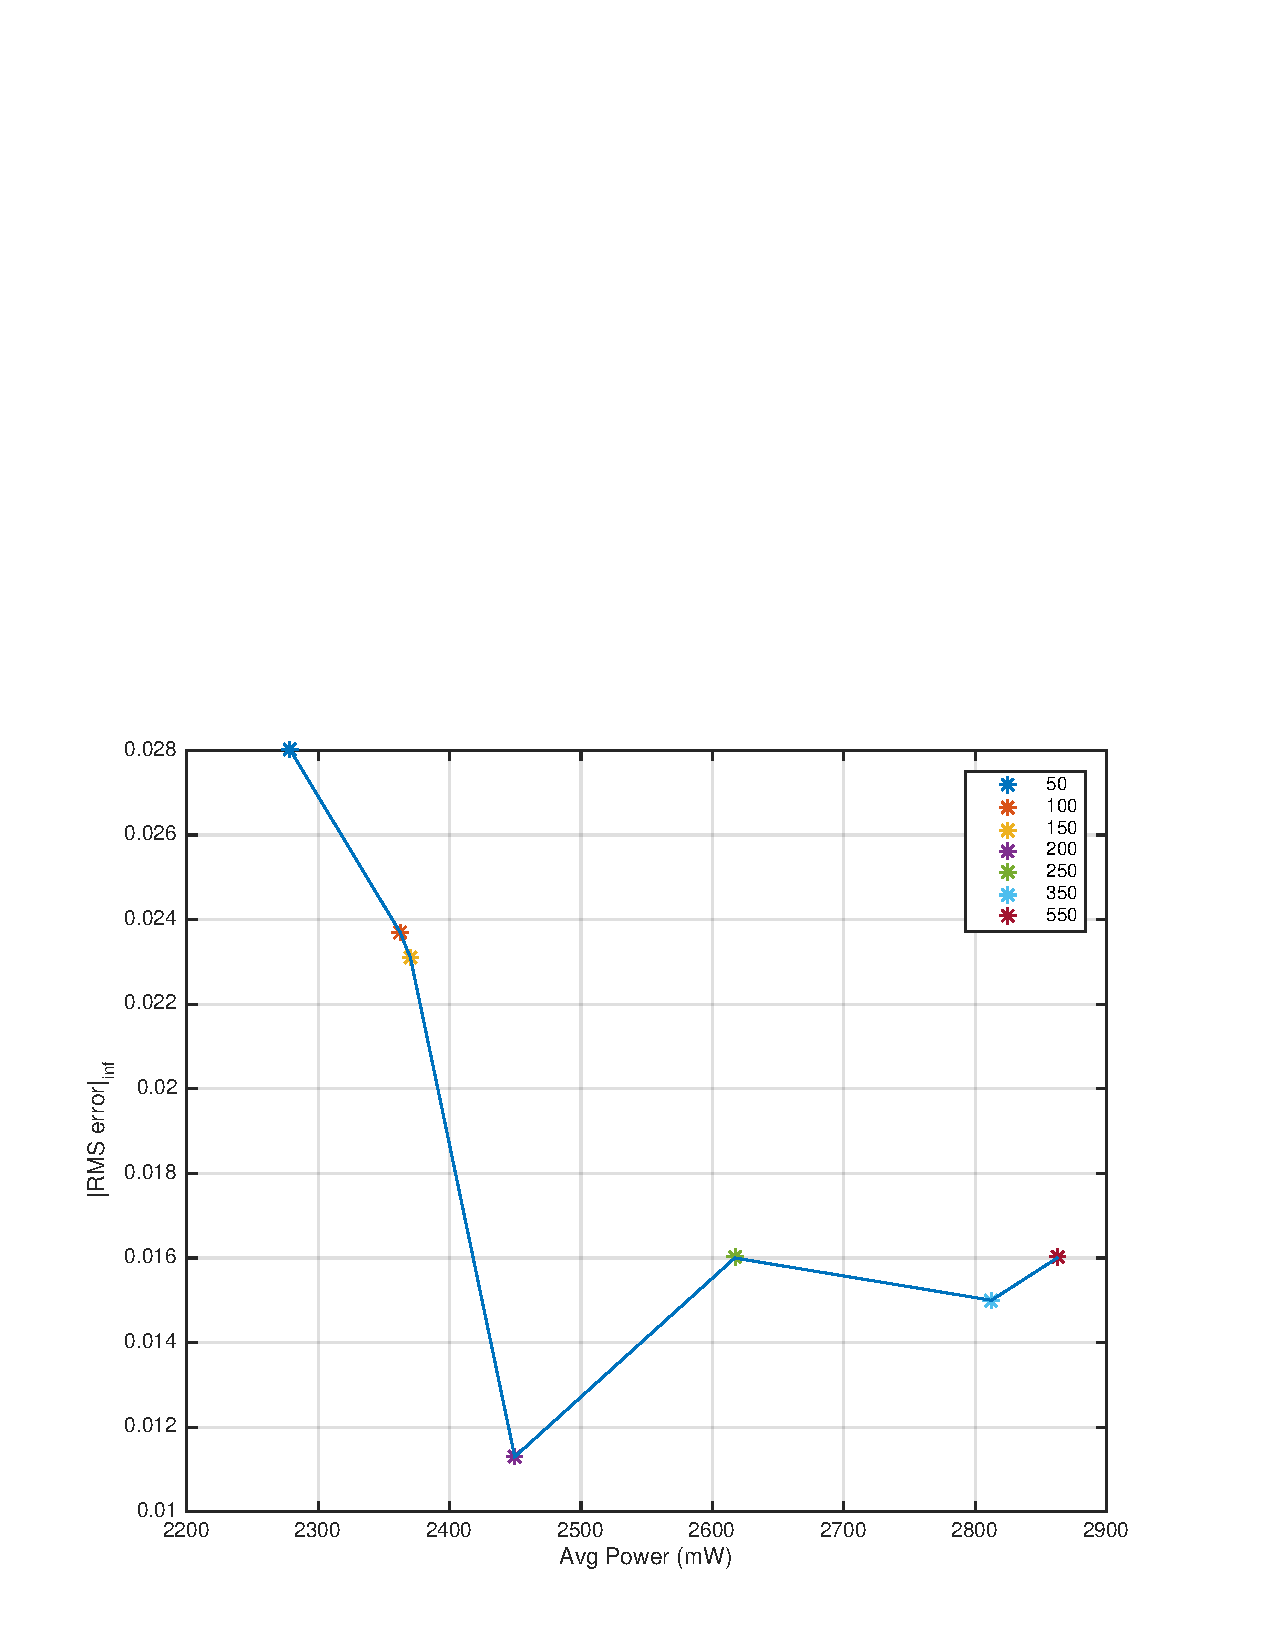
\includegraphics[width=0.7\linewidth]{figures/errVsPower}
	\caption{Error-delay curve for the FAST corner detector running on the Odroid U3}
	\label{fig:fastErrVsPower}
\end{figure}

Our second example is a more complete perception tool chain shown in Fig.~\ref{fig:chain}.
\begin{figure}[t]
	\centering
	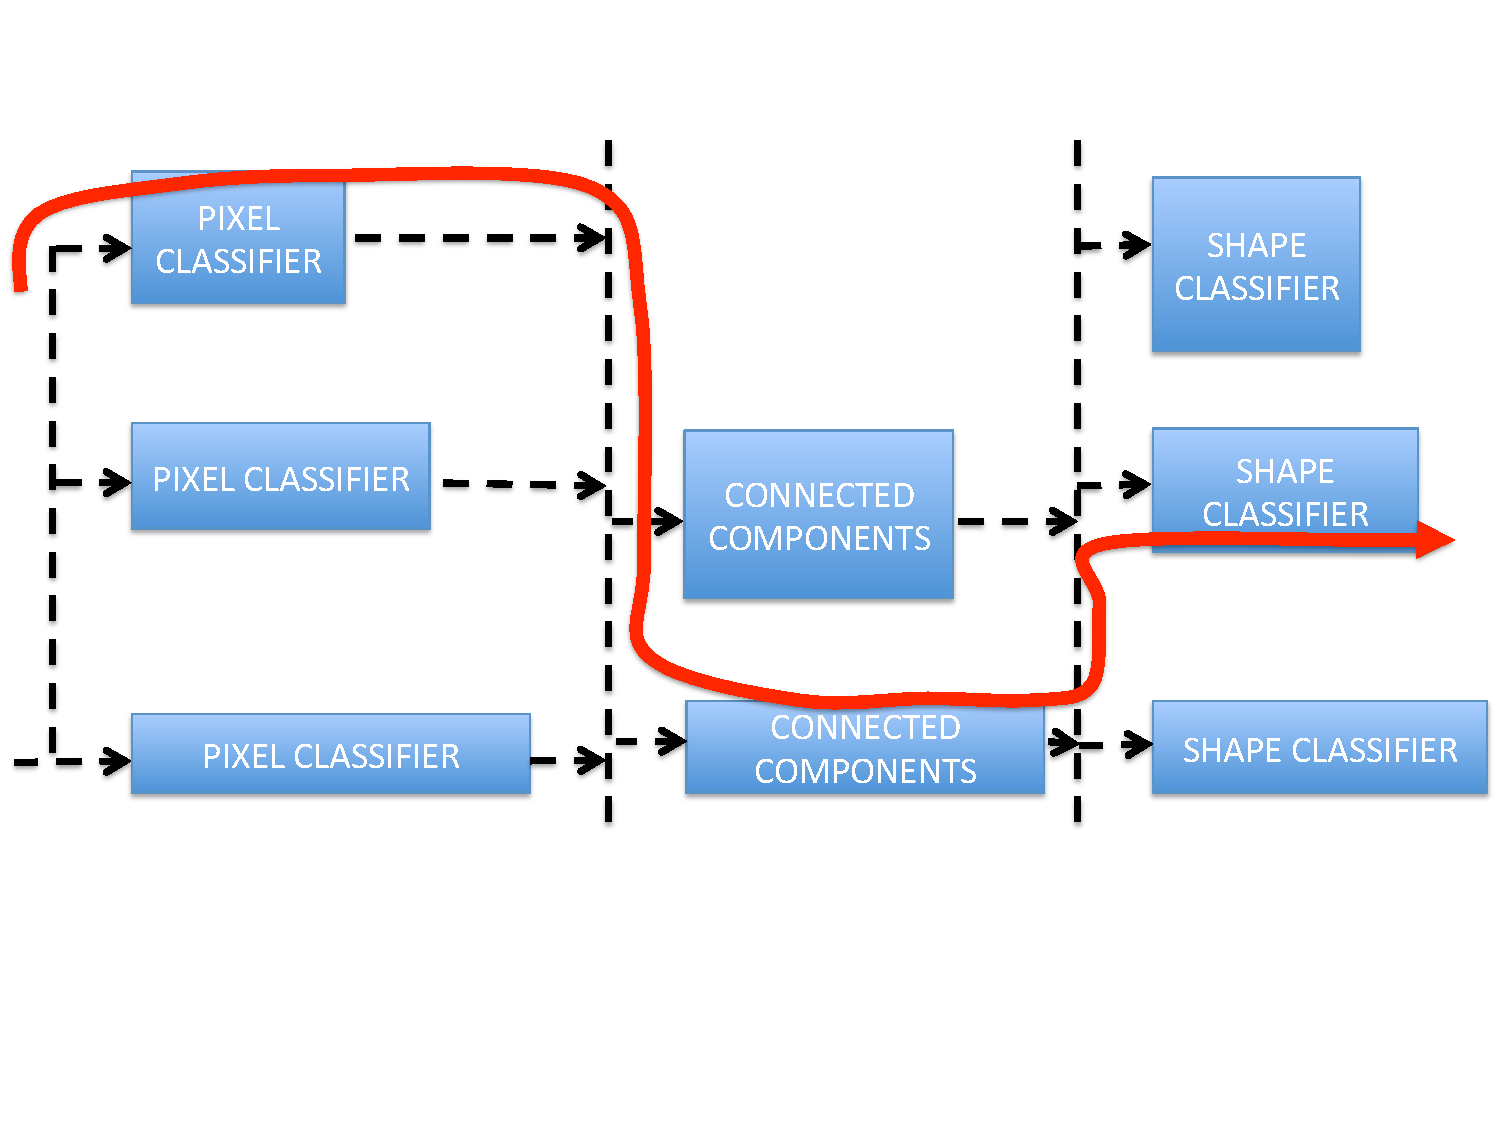
\includegraphics[width=0.7\linewidth]{figures/chain}
	\caption{Visual perception toolchain for object detection. Each component presents error vs runtime options: height of a block indicates output error, while width indicates runtime. The red path indicates one particular execution path which trades error for runtime at each stage.}
	\label{fig:chain}
\end{figure}
The tool chain takes in a video stream and tracks an Object Of Interest (OOI) across the frames.
The pixel classifier assigns to each pixel of the image (after potential pre-processing) the probability of its being a pixel of interest, i.e., of belonging to an OOI. 
A binary image is then obtained which assigns the value 1 to determined pixels of interest, and 0 to all others. 
A Connected Components (CC) algorithm is run on the binary image to segment its 1-valued pixels into disconnected objects.
A shape classifier is then run on each object to determine whether it is an object of interest or not.
The classifiers are machine learning algorithms that need to be trained on a training set before being used in the application.
In our implementation of this chain, the specific algorithms and their knobs are as follows:
the pixel and shape classifiers are Gaussian Mixture Models (GMMs), whose knob is the number of Gaussians in the mixture.
The connected components algorithm has a two-valued knob to choose between a 4-connected and 8-connected component implementation.
Thus the knob for the entire chain is $K$ = (\#Gaussians for pixel classifier, \#neighbors for CC, \#features for shape classifier), and has a total of $3 \times 2 \times 2 = 12$ values.
Note that for any given algorithm in the chain, the relation between knob value and quality of output is not necessarily monotonic. 
Like all machine learning algorithms, it will depend on the actual data set.
The same is a fortiori true of the quality of the output of the entire chain.

Fig.~\ref{fig:chainErrorDelay} shows the \emph{perception error}-delay curve for the object detection chain.
The perception error is the difference between the estimated centroid of the OOI and the true centroid of the OOI.
If the chain fails at finding the object in the image, we assign that image a constant error drawn from the errors found on other images.
For each point on the curve, first the classifiers were trained with the relevant knob values, and then run on the test set to obtain the $(\delta,\epsilon)$ values.
The plotted error value is the average error over all images in the test set.
The fact that the error \emph{increases} in some points despite increasing computation time can be explained by the remark made earlier: namely that the effect of a knob value is not necessarily monotonic on quality.
Moreover, the effect of a change to one algorithm of the chain might outweigh changes to other algorithms.
This makes profiling all the more important.

This curve can then be turned into an estimate error-delay curve by incorporating it into an estimation algorithm.
\begin{figure}[t]
	\centering
	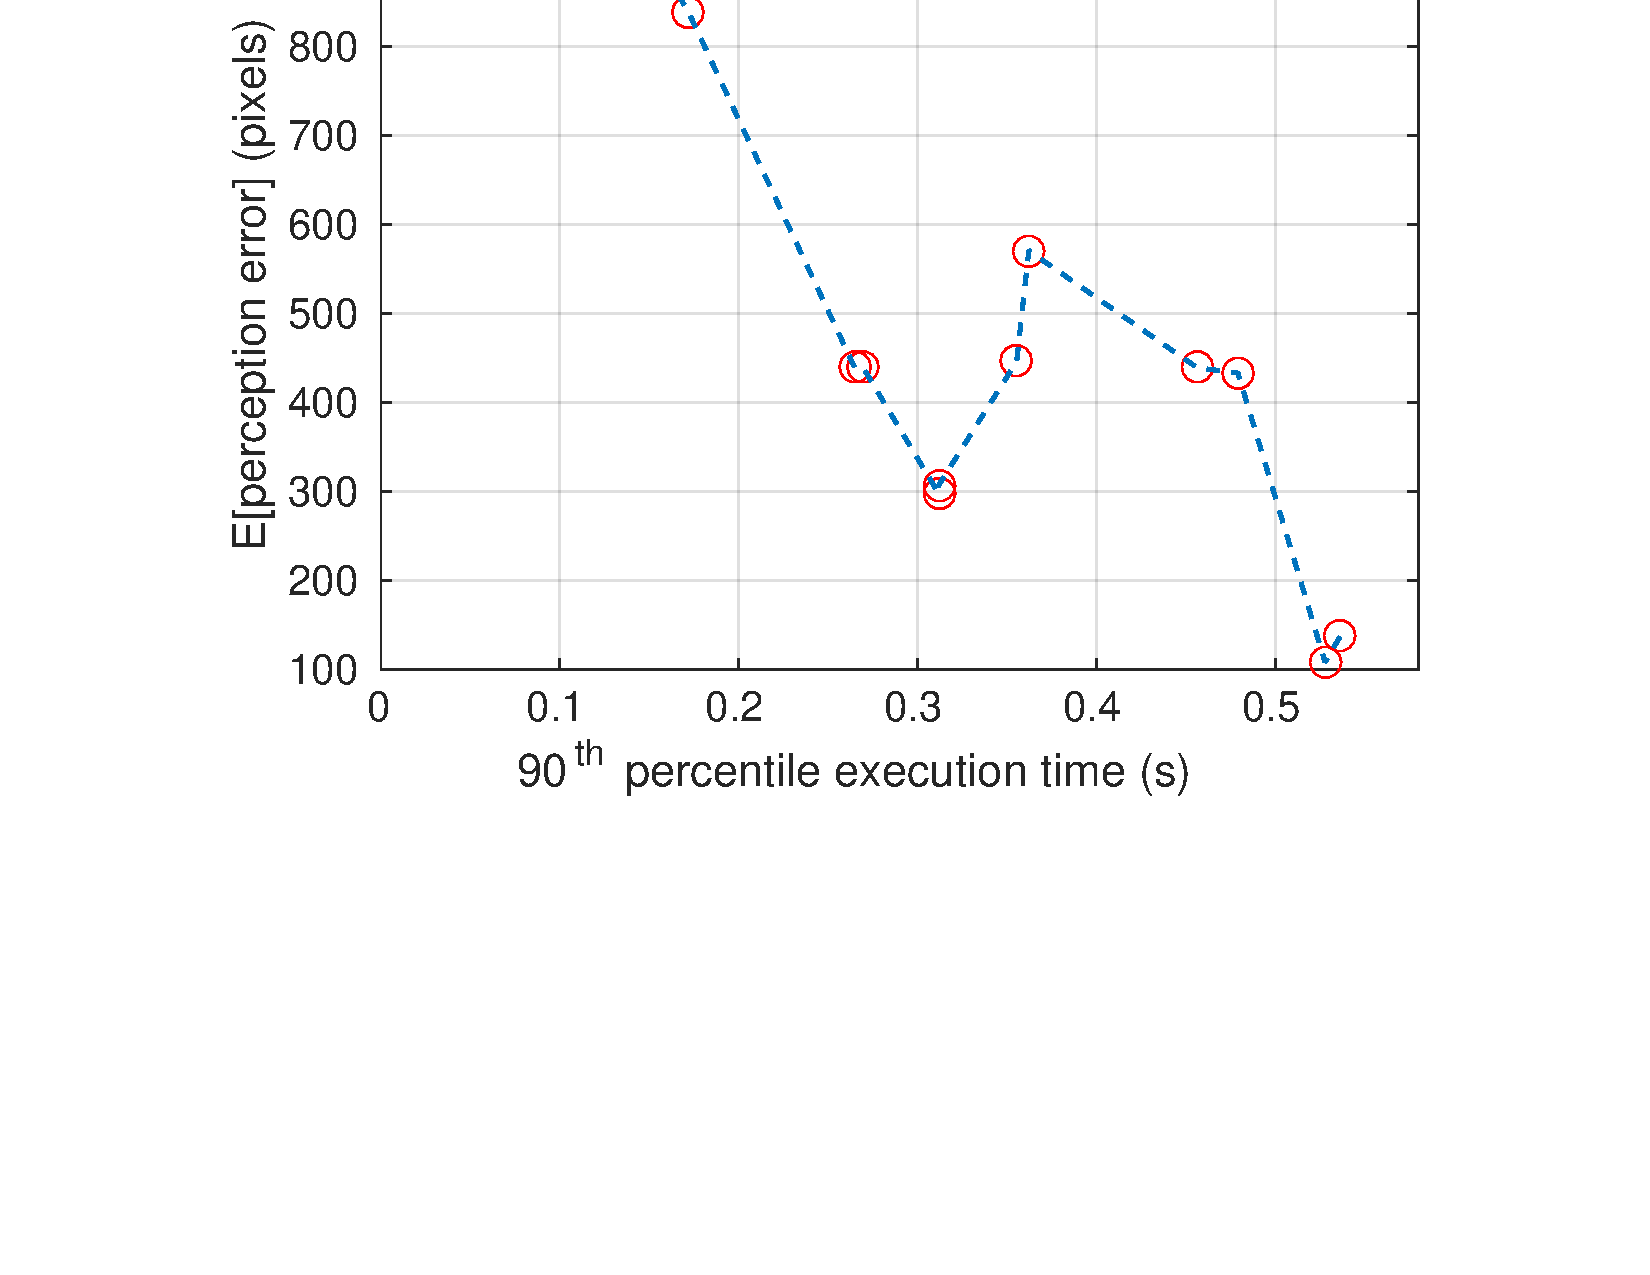
\includegraphics[width=0.7\linewidth]{figures/chainErrorDelay}
	\caption{Perception error vs Delay curve for the chain of Fig.~\ref{fig:chain}}
	\label{fig:chainErrorDelay}
\end{figure}
More generally, such curves can be obtained for a given state estimator by identifying the knobs that control the quality and runtime of the estimator, and profiling the estimator's code at the various values of the knobs.
In effect, this gives us several Estimator tasks, each with a different utility. 
I.e., each such task strikes a different balance between computation time and quality of estimate.
At time step $k$, the controller schedules the task with the best trade-off for step $k+1$, in the sense of optimizing the cost function in Eq.??

